\documentclass{report}
\usepackage[T1]{fontenc}
\usepackage{color}
\usepackage{amssymb}
\usepackage{mathrsfs}
\usepackage{amsmath}
\usepackage{eurosym}
\usepackage{graphicx}
\usepackage{textcomp}
\usepackage{listings}
\usepackage{epigraph}
\usepackage{setspace}
\usepackage[some]{background}
\usepackage{gensymb}
\usepackage{tikz}
\usepackage{fancyhdr}
\usepackage[margin=0.9in]{geometry}
\usepackage[english]{babel}
\definecolor{purple}{rgb}{0.5,0,0.41}
\lstset{
float=hbp,
language=java,
basicstyle=\ttfamily\small\color[rgb]{0.20,0.20,0.20},
upquote=true,
aboveskip={1.5\baselineskip},
columns=fullflexible,
showstringspaces=false,
extendedchars=true,
breaklines=true,
showtabs=false,
showspaces=false,
frame=trbl, 
tabsize=4,
numbers=left,
breakautoindent=true,
extendedchars=true,
showstringspaces=false,
identifierstyle=\ttfamily,
frameround=ffff,
captionpos=b,
xrightmargin=0cm,
xleftmargin=0cm,
identifierstyle=\ttfamily,
keywordstyle=\bf\color[rgb]{0.5,0,0.41},
commentstyle=\color[rgb]{0.25,0.37,0.75},
stringstyle=\color[rgb]{0.16,0,1},}
\pagestyle{fancy}

\begin{document}
\renewcommand{\chaptername}{Part}
\renewcommand{\thechapter}{\Roman{chapter}}

%\usepackage{lmodern}
%\usepackage{xspace}
%\usepackage{hyperref}
%\usepackage{fancyhdr}

% header style
\pagestyle{fancy}
\renewcommand{\headrulewidth}{1pt}
\fancyhead[L]{March, $1^{st}$ 2015}
\fancyhead[R]{\textbf{Reference :} model-checking.archi - Version 3}

% Redefine the plain page style
\fancypagestyle{plain}{%
  \fancyhf{}%
  \renewcommand{\headrulewidth}{1pt}
  \fancyhead[L]{March, $1^{st}$ 2015}
  \fancyhead[R]{\textbf{Reference :} model-checking.archi - Version 3}
  \fancyfoot[C]{\thepage}
}

% title page
\definecolor{sup_strip_color}{rgb}{0.70,0.70,0.70}
\definecolor{inf_strip_color}{rgb}{0.00,0.00,0.00}

\DeclareFixedFont{\bigsf}{T1}{phv}{b}{n}{0.7cm}

\makeatletter                       
\def\printauthor{%                  
    {{\large \@author}}}              
\makeatother

\author{Zohour \textsc{Abouakil} ~\\ Sofia \textsc{Boutahar} ~\\ David \textsc{Courtinot} ~\\ Xiaowen \textsc{Ji} ~\\ Fabien \textsc{Sauce}}

\begin{titlepage}

\newgeometry{left=1cm,right=4cm,bottom=0cm}
\begin{tikzpicture}[overlay,remember picture]
% the black stripe with the title
\node[
  fill=inf_strip_color,
  anchor=north west,
  text width=\paperwidth,
  text height=2cm,
  text depth=2cm,
  inner xsep=1cm,
  font=\color{white}\bigsf 
  ] 
 at ([yshift=-2.5cm]current page.north west) (blackrect) {Architecture document - Version 3};
% the khaki stripe
\path[fill=sup_strip_color] 
  (blackrect.north west) rectangle ++(\paperwidth,2.5cm);
\end{tikzpicture}

\vspace*{4.5cm}

\noindent
\begin{minipage}{0.35\linewidth}
    \begin{flushright}
        \printauthor
    \end{flushright}
\end{minipage} \hspace{15pt}
%
\begin{minipage}{0.02\linewidth}
    \rule{1pt}{175pt}
\end{minipage} \hspace{-10pt}
%
\begin{minipage}{0.6\linewidth}
\vspace{5pt}
\newenvironment{test}{\begin{center}}{\end{center}}
\hspace{10pt}
\begin{minipage}{\linewidth} 
\textbf{Reference :} model-checking.archi ~\\
March, $1^{st}$ 2015
\end{minipage}
\end{minipage}

\vspace{8cm}
\begin{minipage}{0.20\linewidth}
    \begin{flushright}
       
        \begin{tabular}{ll}
	 \textit{Signatures} & \\
			& \textbf{Project manager - Zohour \textsc{Abouakil} :} \\
            & \textbf{Quality responsible - David \textsc{Courtinot} :} \\
            & \textbf{Customers - David \textsc{Doose} - Julien \textsc{Brunel} :} \\
        \end{tabular}
    \end{flushright}
\end{minipage}

\end{titlepage}
\restoregeometry
\tableofcontents
\newgeometry{left=2.1cm,right=2.1cm}
\chapter*{Changelog}
\begin{center}
\begin{tabular}{|c|l|l|}
  \hline
  Version & Date & Change  \\
  \hline
  V3 & February $21^{th}$  & fixed the class diagrams, which did not respect the UML standard \\
  & February $21^{th}$ & minor changes in explications \\
  & February $21^{th}$ & added the CTL part \\
  & February $21^{th}$ & changed the code presentation for it to be printable in black and white \\
  & February $21^{th}$ & changed most resources from png to pdf for better quality and scalability \\
  & February $22^{th}$ & added the merge part \\
  \hline
  V4 & March $1^{st}$ & completed the merge part with patterns and labelizers \\
 \hline
\end{tabular}
\end{center}
\chapter{Context}

\section{Objectives and motivations}

\paragraph{}
\hspace{4mm}Embedded systems are most often critical systems and must be as robust as possible to avoid critical failures which could have dramatic consequences.
Hence, many researches are done in order to build tools that would help to ensure the good properties of an embedded system source code and compensate potential human
failure. The model checking, which consists in asserting properties on a model thanks to graph search algorithms (for example), is one of those fields that can be
applied to this matter. In this project, we are trying to build a model checker working on C++ code which takes the source code as an input and is transformed a few times
in various abstract representations to end with a graph model that we are able to send to a model checker.

\section{Definitions}

\subsection{AST - Abstract Syntax Tree}

\paragraph{}
\hspace{4mm}The AST is an abstract (and low-level) representation of the code. It is a tree data-structure which describes the code in a purely syntactic point of view. As an example,
you can see below a simple C/C++ code and its AST representation. The AST is provided by the Clang API, which performs the first step of our
transformation chain.

\begin{lstlisting}[language=java]
void fun(int &a) {
    ++a;
}

int main(int argc, char* argv[]) {
    int num = 10;
    if (num > 5)
        fun(num);
    
    return 0;
}
\end{lstlisting}
\begin{center}
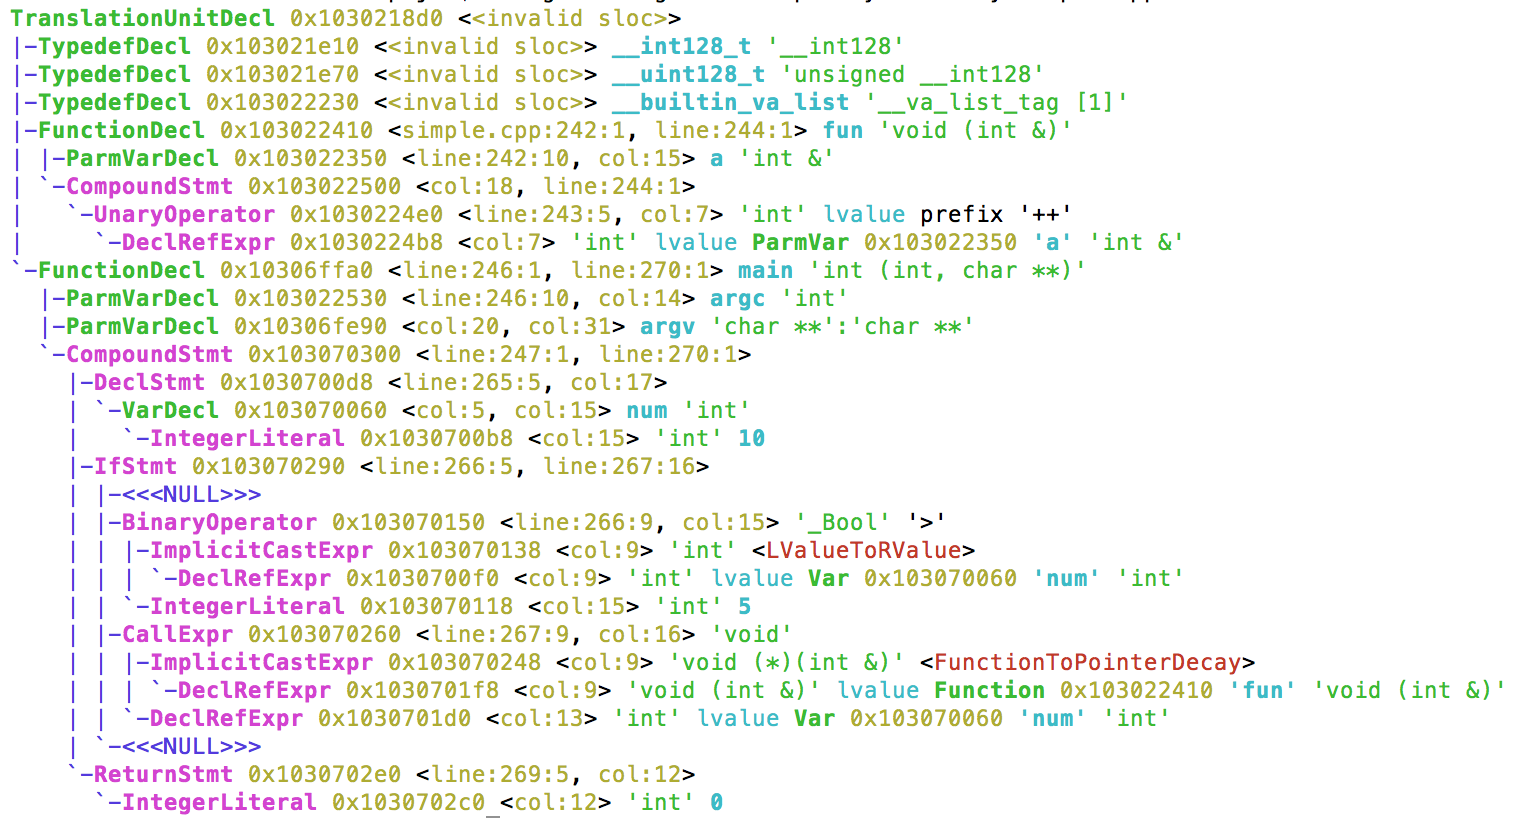
\includegraphics[scale=0.6]{data/ast}
~\\~\\Figure I.1 - The AST corresponding to the above code
\end{center}

\subsection{CFG - Control Flow Graph}

\paragraph{}
\hspace{4mm}The CFG is a graph representing all the possible execution paths (with some restrictions, for example
we won't create several nodes for a single expression even if in reality an expression should be a graph).
As an example, you can find below the CFG generated by a  do while statement in an if statement.

\begin{center}
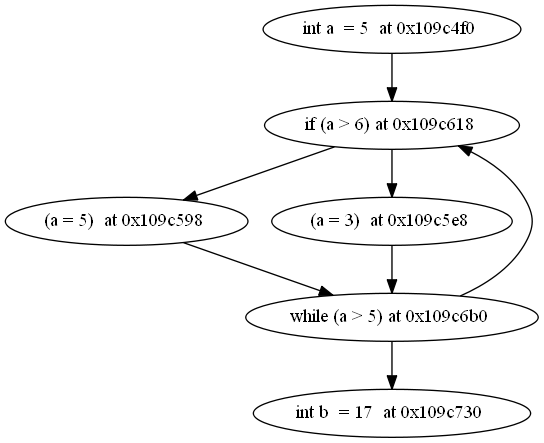
\includegraphics[scale=0.4]{data/doWhile}
~\\~\\Figure I.2 - An example of CFG
\end{center}

\subsection{CTL - Computation Tree Logic}

\paragraph{}
\hspace{4mm}CTL is a way of representing temporal logic expressions on a graph or a tree. For example, it can
express properties such as \textit{<< All the paths starting from every node verifies the predicate p >>}.

\chapter{AST and CFG representations}

\paragraph{}
\hspace{4mm}After studying the Clang API, we came to the conclusion that the AST is a much more low-level representation of the program than the CFG. 
Indeed, the atom for a CFG is what is generally called a \textit{statement} whereas the simplest instruction
gives an AST representation composed of multiple nodes. We also found it difficult to handle the parsing and the linking of the graph nodes at the same time.
Thus, we have chosen to transform the AST into a series of higher-level objects than the original nodes, which will be converted
in nodes of the CFG.

\begin{center}
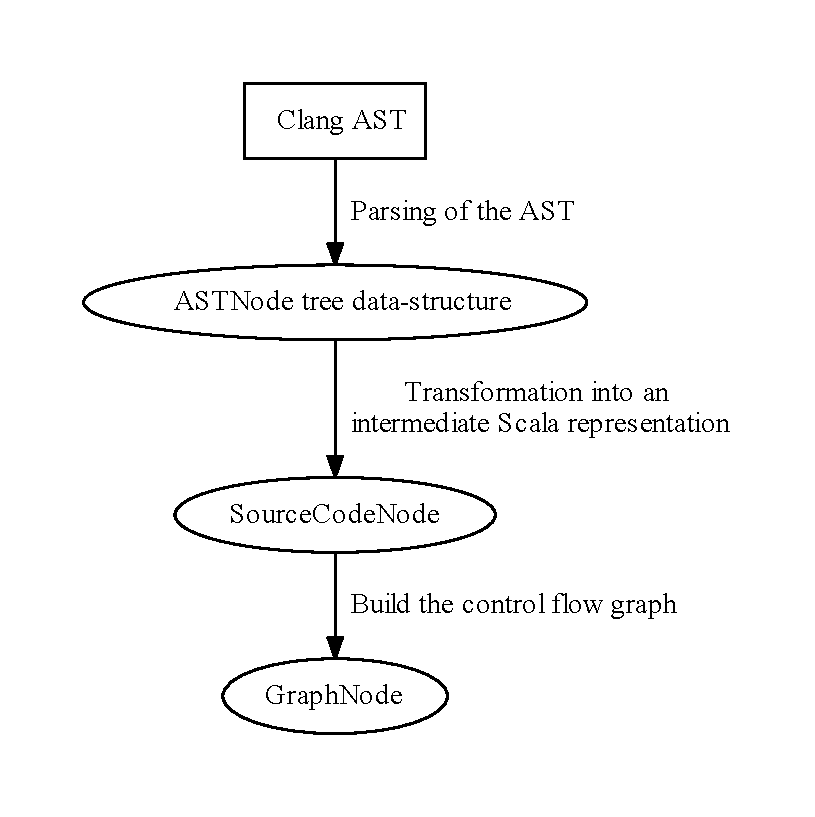
\includegraphics[scale=0.5]{data/transform_chain}
~\\~\\Figure II.1 - Transformation chain we are going to present
\end{center}

\section{Intermediate representation of the Clang AST}

\subsection{Parsing the Clang AST file}

\paragraph{}
\hspace{4mm}At first, we have considered using XML parsing libraries to parse the XML version of the Clang AST. However, 
this type of output is no longer supported by the newest versions of the Clang compiler and all the existing tools
provide partial support at best. Hence, we decided using the regular AST file and parse it line by line 
with a custom parser.

\paragraph{}
\hspace{4mm}We have identified three main kinds of nodes in the AST. Each one is associated to a specific class which extends ASTNode :

\vspace{1.5mm}
\begin{itemize}
\item nodes consisting in an type name, an id, a code pointer pointing the relevant lines of the code and some
metadata that depend on the type of the node. These are represented by the ConcreteASTNode class.\vspace{1mm}
\item < < <NULL> > > children, represented by the NullASTNode class.\vspace{1mm}
\item other kind of nodes, prior to class declaration for example. These are represented by OtherASTNode.\vspace{1mm}
\end{itemize}

\paragraph{}
\hspace{4mm}The file will be parsed and converted in a tree data-structure which nodes are of type ASTNode. The ASTNode objects
will then be converted in Stmt or Decl accordingly to the class hierarchy we present in the next part.

\begin{center}
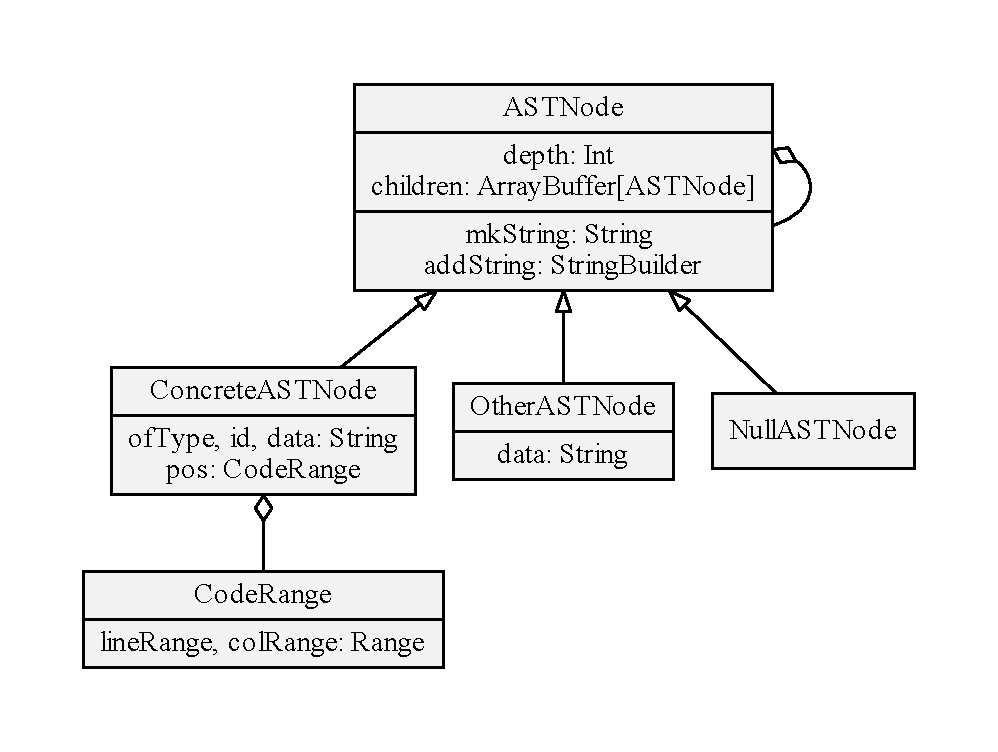
\includegraphics[scale=0.6]{data/AST_classes}
~\\~\\Figure II.2 - Class hierarchy for the output format of the ASTParser
\end{center}

\subsection{From ASTNode to SourceCodeNode}

\paragraph{}
\hspace{4mm}The SourceCodeNode class represents a tree data-structure which is still close enough to the AST 
but with a higher abstraction, and some removed low-level information.

\subsubsection{Decl class hierarchy}

\paragraph{}
\hspace{4mm}For the Decl part,  which represents the different kinds of declarations in the code, we did not have too much trouble and just had to associate each high-level Clang Decl class to a Scala class extending
our Decl class, as it is shown in the previous figure.

\subsubsection{Stmt part}

\paragraph{}
\hspace{4mm}Stmt is a Clang asbtraction of a statement in a program (any expression, any flow-control structure). As it was not presented as a priority by the client, we have decided to skip the C++ object oriented 
part in order to focus exclusively on the imperative part. Inspired by the Clang API, we came up
 with the following class hierarchy :

\begin{center}
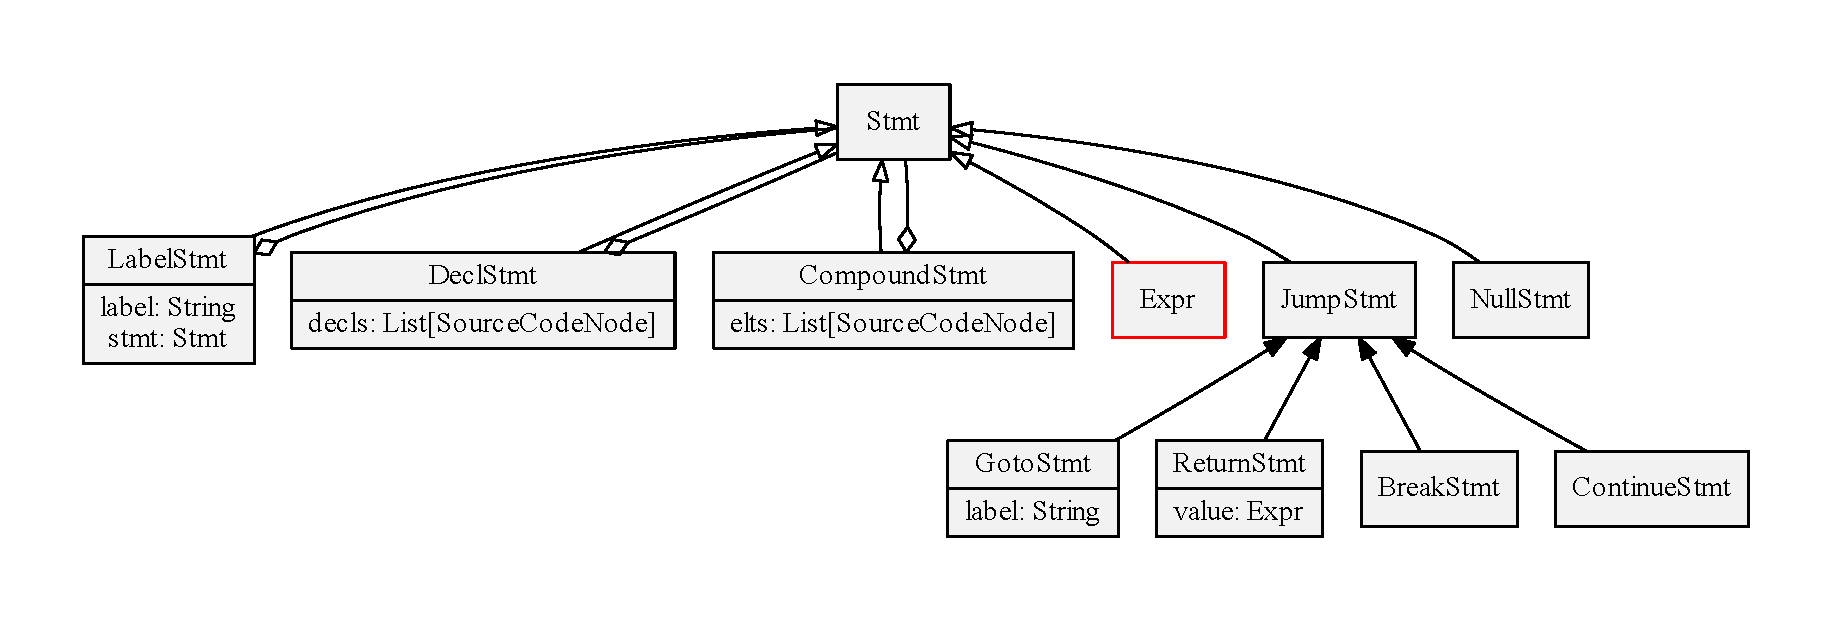
\includegraphics[scale=0.5]{data/basic_Stmt_classes}
~\\~\\Figure II.3 - Representation of the most classes statements
\end{center}

\begin{center}
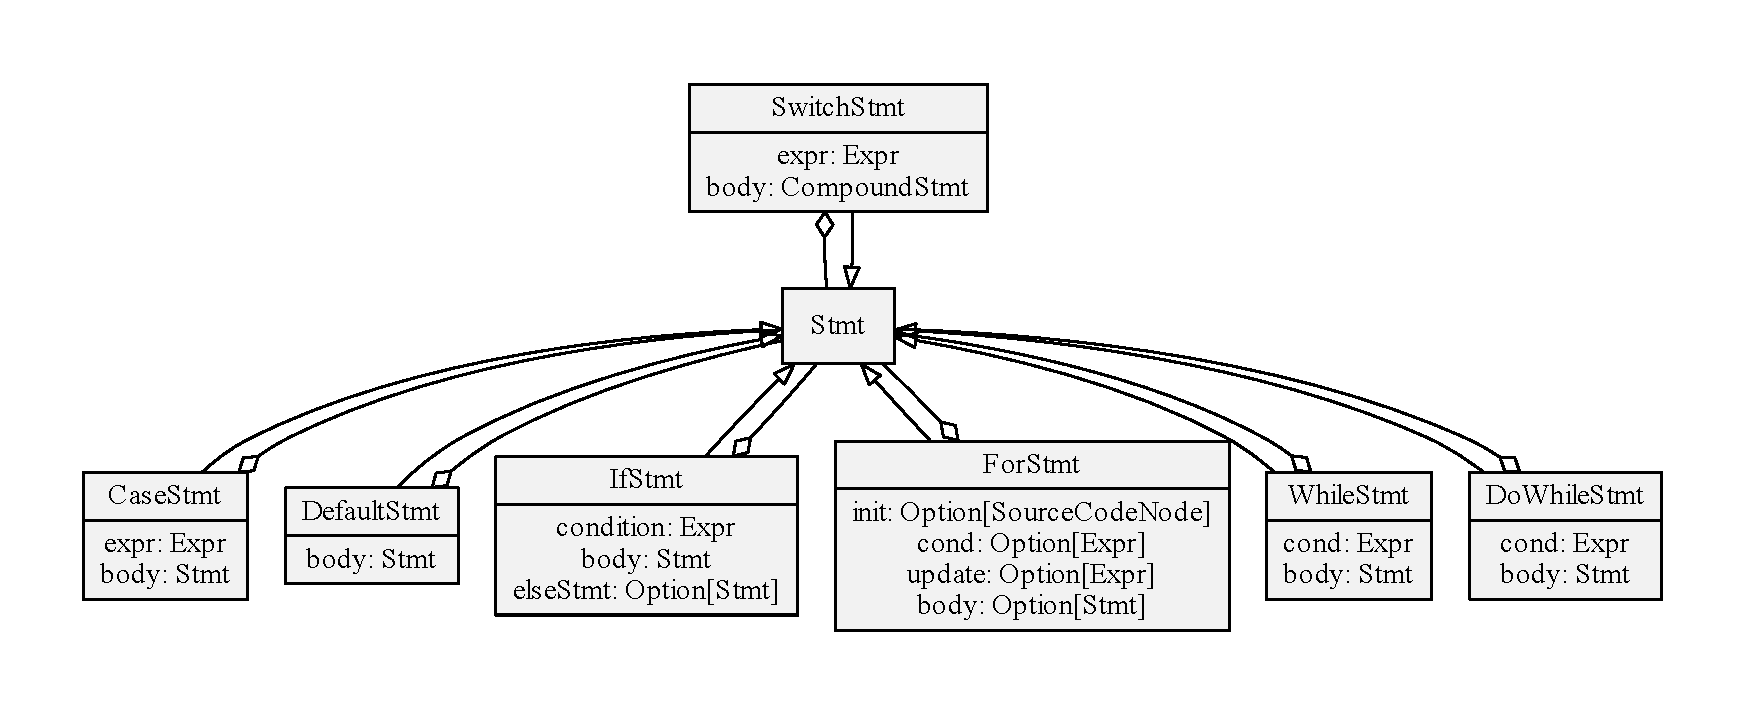
\includegraphics[scale=0.5]{data/flow_control_Stmt_classes}
~\\~\\Figure II.4 - Flow-control structures
\end{center}

\begin{center}
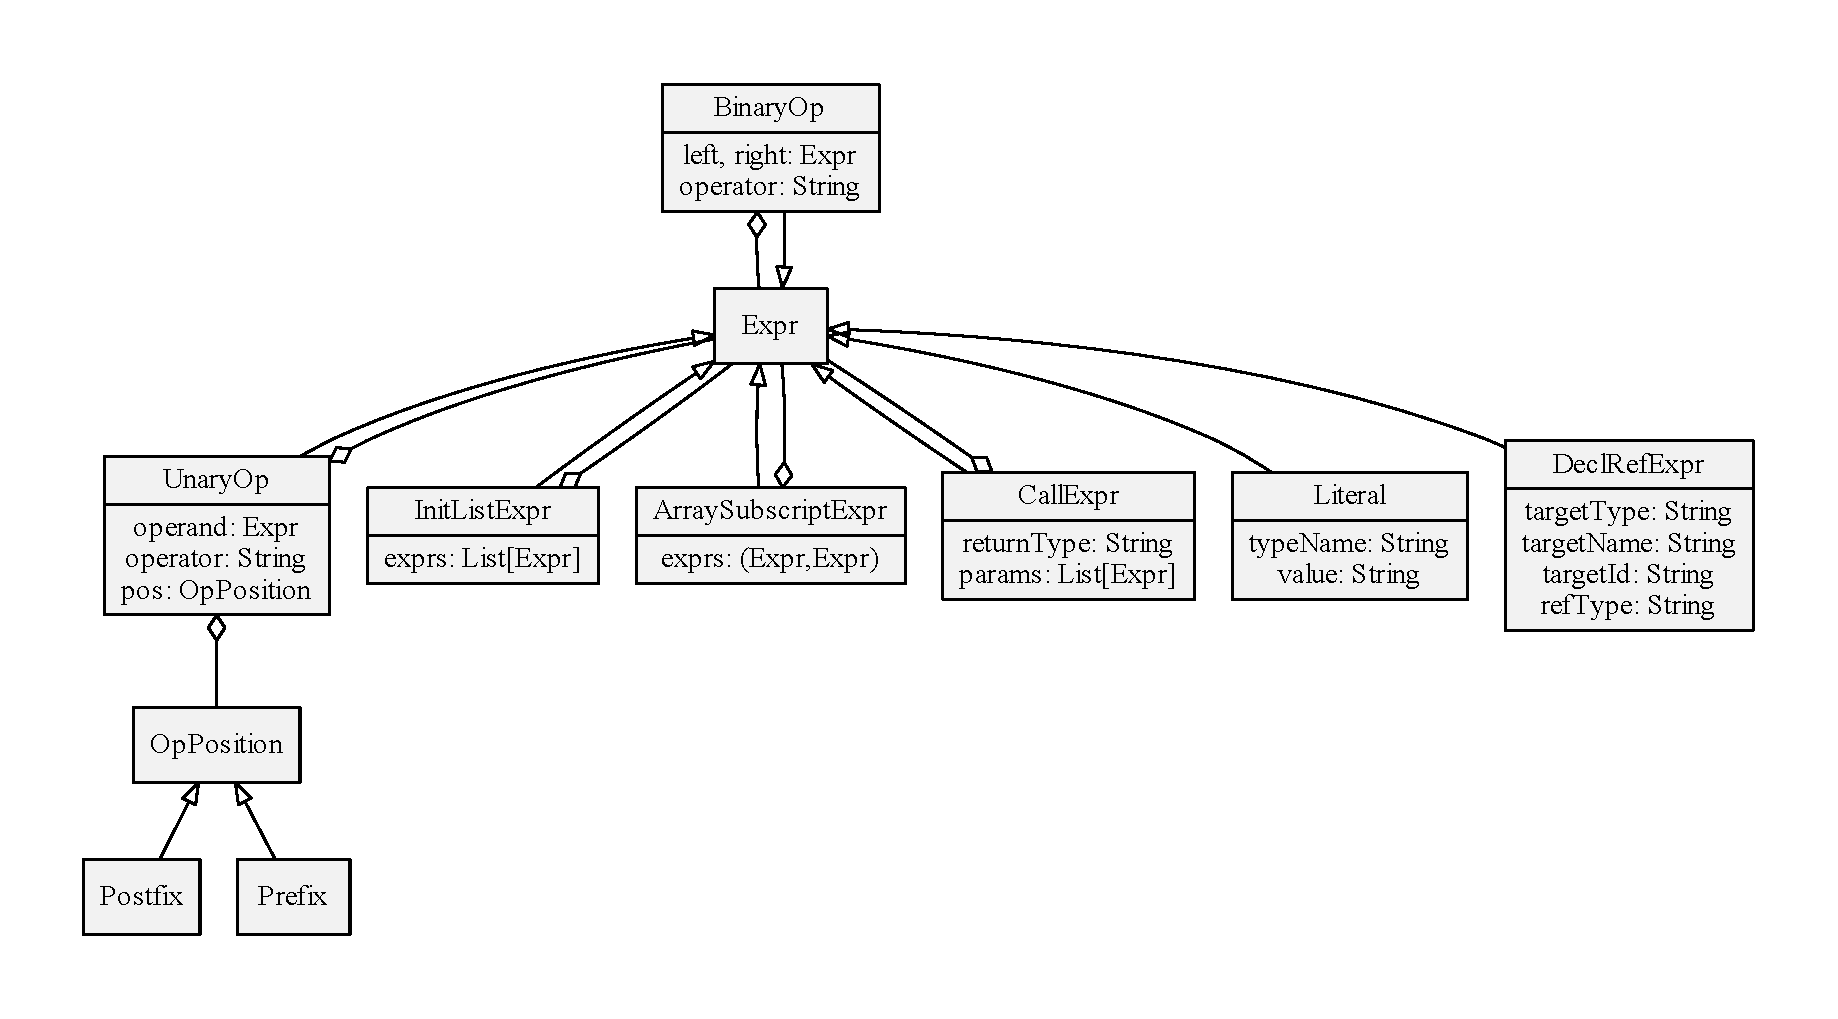
\includegraphics[scale=0.5]{data/Expr_classes}
~\\~\\Figure II.5 - Detail of the Expr class hierarchy
\end{center}

\paragraph{}
\hspace{4mm}Note that our model does not strictly represents a C++ code. For example, we do not prevent a \textit{if} to contain the instruction \textit{break}
(among other inaccuracies ...). We felt that this kind of refinement would unnecessarily complicate the task without adding anything more to the CFG analysis. 
Since the code is already semantically checked by the Clang compiler and given our future needs, we thought it would be wiser to aim for a simple model.

\subsubsection{Important notes}

\vspace{1.5mm}
\begin{itemize}
\item To accurately represent the CFG of our input programs, we should take into account the fail-fast mechanism in the evaluation of boolean conjunctions/disjunctions.
The importance of this mechanism for our project is illustrated in the figure below.\vspace{1mm}
\item However, since the evaluation's order of the expressions is not completely specified specified in C++ (unlike Java which evaluates from left to right),
we will ignore that even if it will surely change the result for certain kind of treatments when some expressions contain side-effect sub-expressions
 (increment, assignments...).\vspace{1mm}
\end{itemize}

\begin{center}
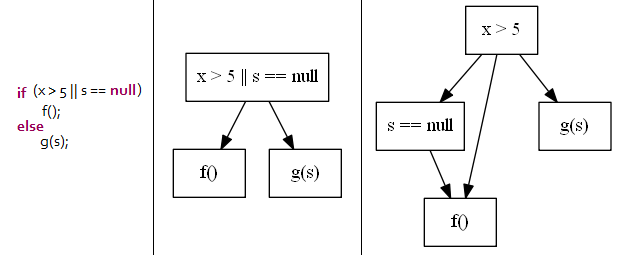
\includegraphics[scale=0.7]{data/fail-fast}
~\\~\\Figure II.6 - On the left, the associated code. On the center, we didn't take into account the fail-fast for the CFG, and finally on the right we consider the fail-fast
\end{center}

\paragraph{}
\hspace{4mm}Just to see what we are losing by ignoring that kind of things is illustrated in the figure above : if we try to
assert the property \textit {<< variable s is always initialized when g(s) is called >>}, the first CFG will not allow us to conclude
(or it will conclude \textbf {true}, erroneously) while the second allows us
to state that there are executions, according to the value of x,
where $g$ is called with an uninitialized parameter
(assuming that the left son is always a successful test and the right son is a failed test). It is not really a problem, as
we could argue that it is fine to use fail-fast most of the times but that it is safer not to use it for a critical program.

\paragraph{}
\hspace{4mm}Finally, we chose to make all the classes as case-classes to enable the powerful Scala pattern-matching.
Most algorithms are recursive, the parsing of the AST being the only exception.

\section{SourceCodeNode to CFG}

\paragraph{}
\hspace{4mm}Considering that Stmt and Decl children classes were partly low-level elements of the code that are not important
in the CFG, we decided to perform a last step of transformation from SourceCodeNode to ProgramNode, which is a simpler and higher level abstraction of the code.
The ProgramNode objects will be the values of the nodes of the actual graph, represented by the class GraphNode[T].

\paragraph{}
\hspace{4mm}GraphNode is actually a generic type, completely independent of all the classes we introduced so far.
It basically represents any oriented unweighted graph. The conversion from SourceCodeNode to
ProgramNode is handled on the fly while constructing the CFG (GraphNode[ProgramNode]), which
consists in creating the links between the various nodes of the graph.

\begin{center}
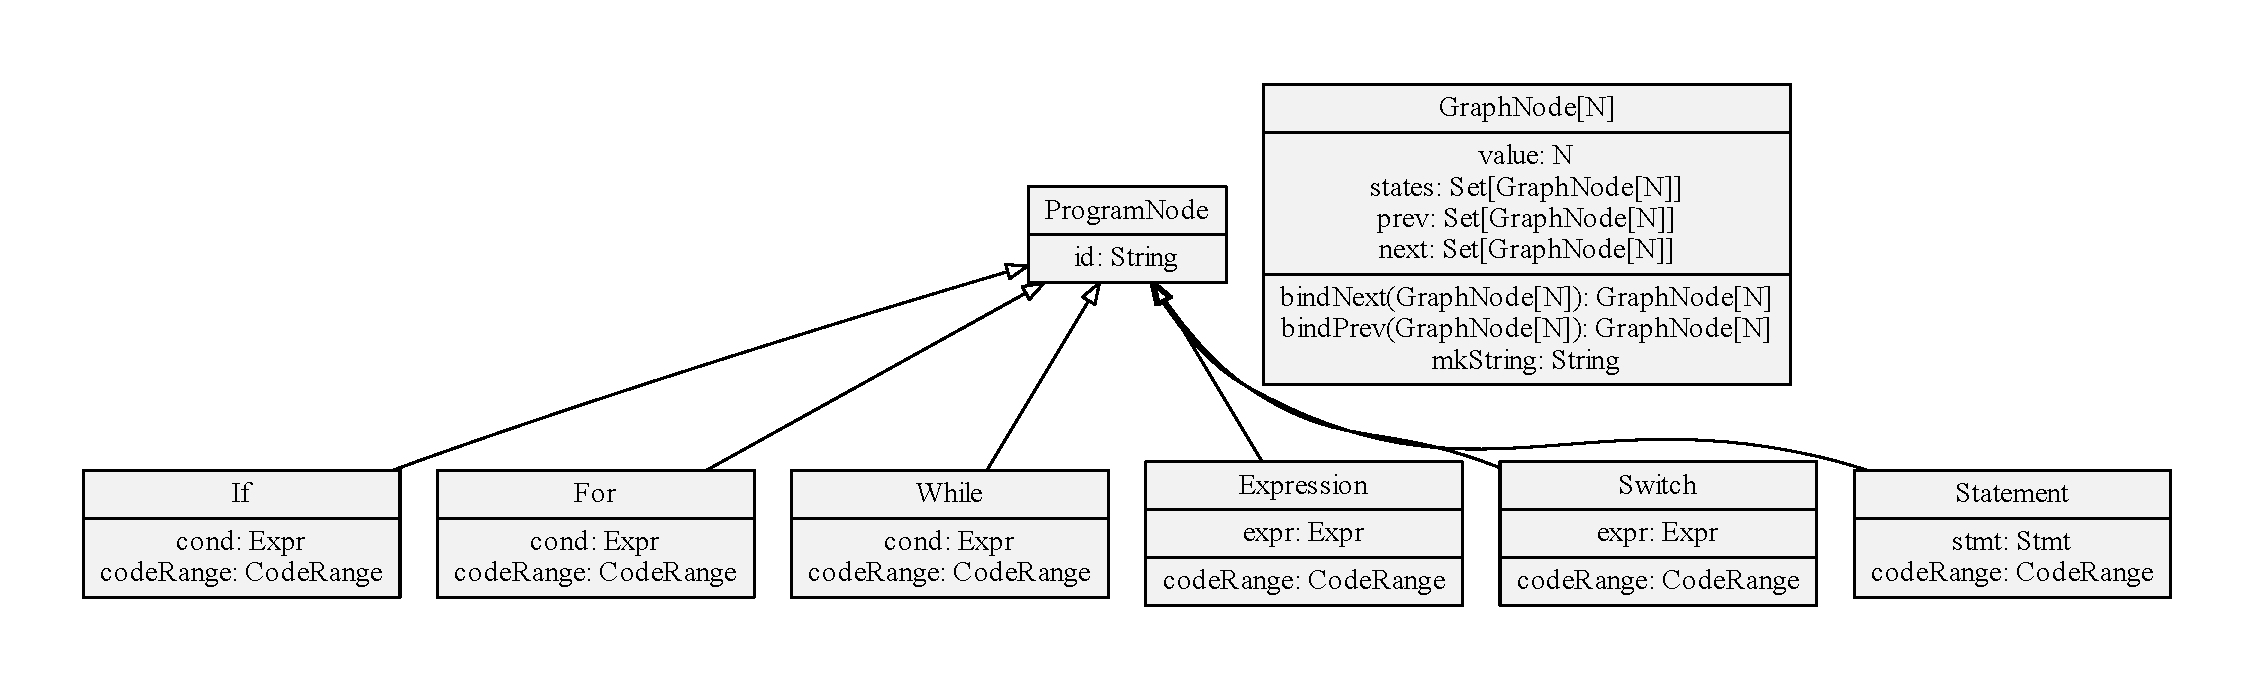
\includegraphics[scale=0.5]{data/CFG_classes}
~\\~\\Figure II.7 - ProgramNode class hierarchy and GraphNode
\end{center}

\chapter{Model checking}

\paragraph{}
\hspace{4mm}The biggest problem we ran into in this part was to achieved a high level of genericity while keeping
a simple architecture, not overly complicated to use for a specific case. We also had to ensure that the architecture is
free of any dependance of any kind with the CFG part.

\paragraph{}
\hspace{4mm}We have identified three kind of entities involved in model checking, each of them corresponds to a generic type :

\vspace{1.5mm}
\begin{itemize}
\item a type M describing the meta-variables. M must extend the MetaVariable trait.\vspace{1mm}
\item a type N describing the values contained by the nodes of the graph (GraphNode[N]). N can be anything.\vspace{1mm}
\item a type V describing the values of the environment. V must extend the Value trait\vspace{1mm}
\end{itemize}

\paragraph{}
\hspace{4mm}One could wonder why we chose using (M <: MetaVariable,V <: Value) instead of 
just (M,V) or (MetaVariable,Value). Here are the advantages of the proposed solution compared to the two others :

\vspace{1.5mm}
\begin{itemize}
\item \textbf{(M <: MetaVariable,V <: Value) vs (M,V)} : more evolutive, we can imagine adding
operations on MetaVariable and Value in the future. This is an advantage for developing new features on the CTL part.\vspace{1mm}
\item \textbf{(M <: MetaVariable,V <: Value) vs (MetaVariable,Value)} : more accurate type. This enables the developer using the model checker to
specialize these generic classes in a more powerful way than it would be in the second case, because the access to specific methods of M and V would be lost.
This is an advantage for using the CTL part in any kind of application.\vspace{1mm}
\end{itemize}

\section{Representation of the environments}

\paragraph{Definition 1}
A \textit{positive binding} is an element of $M \times V$. It associates a meta-variable to a specific value.

\paragraph{Definition 2}
A \textit{negative binding} is an element of $M \times \mathscr{P}(V)$. It associates a meta-variable to a set of illegal values.

\paragraph{Definition 3}
Two bindings are said \textit{in conflict} if :

\vspace{1.5mm}
\begin{itemize}
\item they are two positive bindings $(m,v_1)$ and $(m,v_2)$ such as $v_1 \neq v_2$\vspace{1mm}
\item they are one positive binding $(m,v)$ and one negative binding $(m,V)$ such as
$v \in V$\vspace{1mm}
\end{itemize}

\paragraph{Definition 4}
An \textit{environment} is a set of positive and negative bindings.  An environment 
containing conflicting bindings is noted $\bot$.

\subsection{Methods and class hierarchy}

\paragraph{}
\hspace{4mm}At first, positive and negative bindings were stored in two separate maps but we finally decided 
to use an abstract class MetaVarBinding extended by two case-classes to represent all kinds of bindings and use a single map.
The Environment class contains all the abstract operations between or on environments required by the algorithm :

\vspace{1.5mm}
\begin{itemize}
\item intersection (noted \& in reference to the \& method of the Set trait)\vspace{1mm}
\item removal of a binding (noted - as it is a standard notation for removal in a Scala collection)\vspace{1mm}
\item opposite (noted ! in reference to the logical negation in Scala)\vspace{1mm}
\end{itemize}

\paragraph{}
\hspace{4mm}The following diagram presents the chosen design for environments. Next parts of this section will focus on explaining it all :

\begin{center}
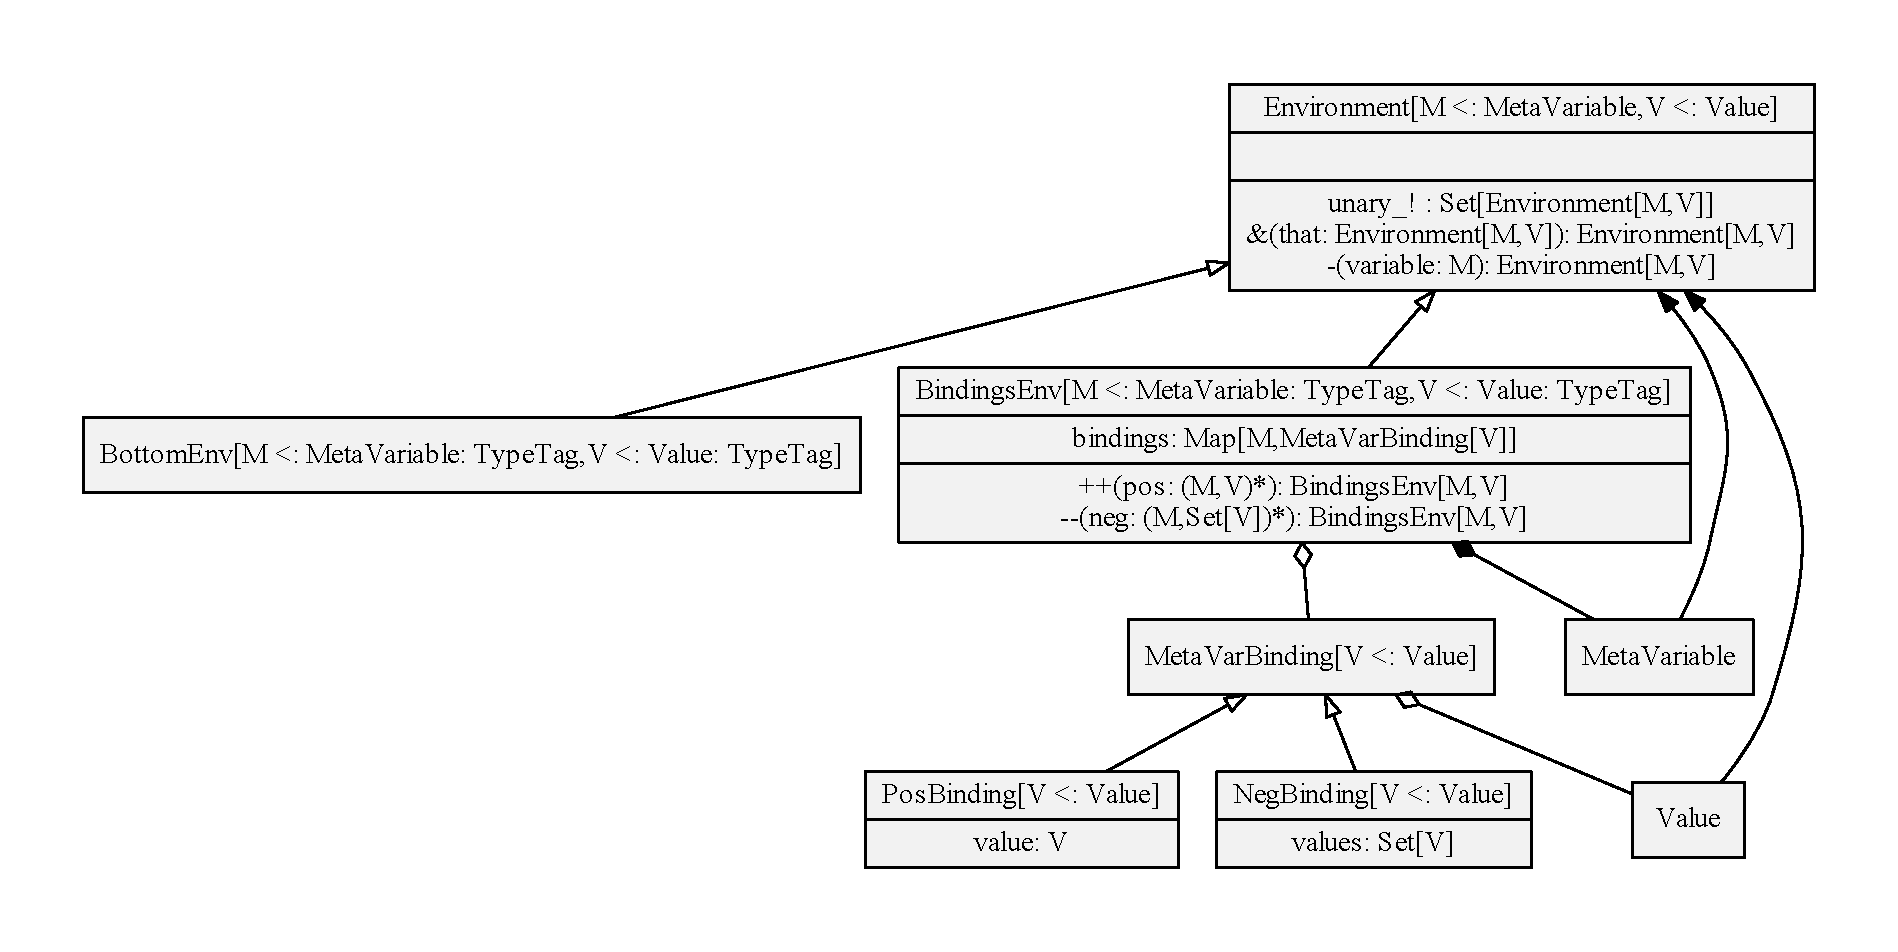
\includegraphics[scale=0.5]{data/Env}
~\\~\\Figure III.1 - Environement class hierarchy
\end{center}

\subsection{The specific case of the $\bot$ environment}

\paragraph{}
\hspace{4mm}The $\bot$ environment was a bit tricky to represent. Indeed, environments depend on generic types
M and V, which implies that Environment must be a generic class. Thus, BottomEnv also must to be generic. However, 
considering the mathematical definition of $\bot$, it would be poor design to represent it with a regular class instead of a singleton.

\paragraph{}
\hspace{4mm}We want all self-contradictory environment of the same generic type to be equal, and if possible we would like two self-contradictory environments of
different generic types not being equal, to keep the type consistency. As Scala does not allow a singleton to be generic (which is quite logical by the way=,
we have had to use reflexivity to implement the singleton pattern without using the \textbf{object} keyword. We also used some implicit definitions to allow nice syntax using 
the Bottom object to fetch the BottomEnv singleton of the appropriate type given the context.

\subsection{Regular environments}

\paragraph{}
\hspace{4mm}Having defined the MetaVarBinding class and its children case-classes, it seems natural to use a single Map[M,MetaVarBinding[V]] map to
represent the bindings. The only real design problem we have got here was the fact that the reflexivity used to solve the BottomEnv problem
was infectious. We have had to use TypeTag(s) in some generic methods and in the BindingsEnv constructor. Thus, any external code
calling the main constructor was forced using TypeTag(s) also. To address this issue, we made the main constructor private and declared and secondary constructor
TypeTag-free creating an empty BindingsEnv object. The user then has to add bindings to this environment using the ++ and - - methods.

\section{CTL expressions}

\subsection{Defining the CTL-V language}

\paragraph{}
\hspace{4mm}There is nothing too difficult here, the class hierarchy is directly derived from the mathematical
definition of CTL operators. The only interesting points are the way of defining generic predicates as well as the way of quantifying variable with the $\exists$ quantifier. These points
will be discussed in the next subsections. Another thing to mention is that we did not define AG, EG, AF and EF as classes but used the mathematical equivalences between the different operators
to define them with implicit declarations using the other operators. This way, we don't have to handle them as particular cases in the model checking algorithm since they are first converted into
a combination of the other operators.

\begin{center}
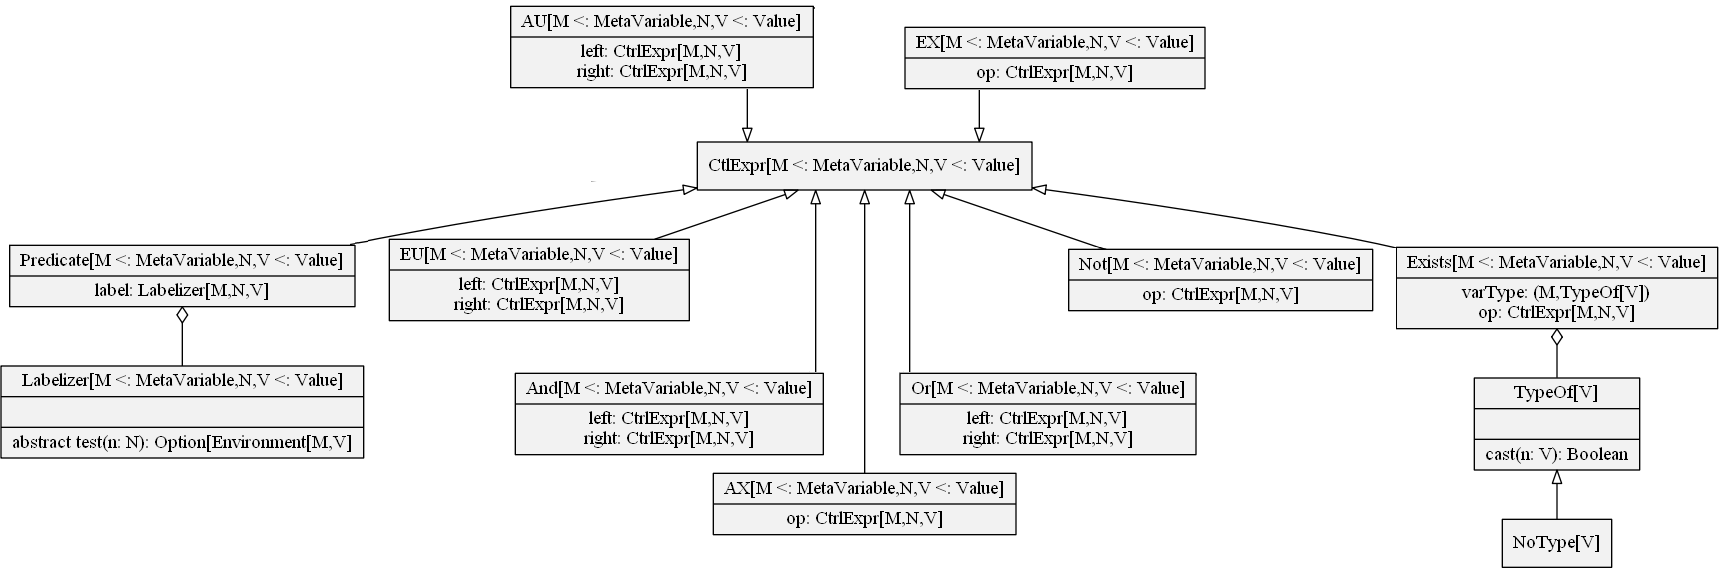
\includegraphics[scale=0.4]{data/CTL_expr.png}
~\\~\\Figure III.2 - CTL expression class hierarchy
\end{center}

\subsection{Predicates}

\paragraph{}
\hspace{4mm}To enable to make generic predicates, we simply defined a generic class Predicate that wraps a Labelizer. A Labelizer
defines a \textit{test} method that takes an object of type N (the type of the GraphNode(s)) and returns an Option[Environment[M,V]].
If the predicate is not verified by the input node, this method must return None, otherwise it returns the set of positive bindings that make the node
match the predicate. This set is possibly empty if the predicate does not involve any meta-variable.

\subsection{$\exists$ quantifier}

\paragraph{}
\hspace{4mm}The $\exists$ quantifier is a bit tricky to define because of the ex\_binding operation defined in the model checking algorithm, which requires
to know the set of all possible values for a given meta-variable. The problem is that the type V may be composed of inconsistent types wrapped by some classes extending V. For example, in the case of the model checking on the CFG,
if X has been assigned a negative binding composed of declarations, then we should not consider that X could possibly be an Expr.

\paragraph{}
\hspace{4mm}To sum up, we must be able to have a type information about the meta-variable at least when encountering the $\exists$ quantifier. Therefore
we introduced the TypeOf class which defines a cast operation. This way, incompatible values will be filtered. This is completely generic as the cast operation is defined by the user depending on its needs.

\section{Model checker}

\paragraph{}
\hspace{4mm}The only interesting thing to mention here is the use of a conversion method for compute the Val set of all possible values.
In order to compute Val, all the nodes of the graph are traversed. For each node, we call the converter that returns all the values of type V a given node is likely to add to the environment. Note that 
a single node can introduce several values in the environment (for example a node f(5,6) would inject 5 and 6 when applying a f(x,y) labelizer), that's why the converter must return a Set[V]. We could have defined
the conversion as an abstract method of the GraphNode, but we thought it was more convenient to do it externally. It is exactly the same difference as
Comparable and Comparator in Java : Comparable defines the comparison operation directly on the class, it is useful when a natural order exists but it enables only one implementation
of the comparison whereas we can define as many Comparator(s) as we want for the same type.

\chapter{Merge}

\section{Choice of M, N and V}

\paragraph{}
\hspace{4mm}Considering the kind of predicates we wanted to use and the types of node we were using (as a recall, type N will be ProgramNode for the CFG), it was kind
of obvious that we would need Expr values in our environment, so we introduced the type CFGExpr, which simply wraps an Expr object. However, it was not so easy determining what other kinds
of values would be required. To solve this question, we thought about the labelizers and properties we wanted to be able to implement to deduce our needs. 
Two important properties led us to introduce types CFGDecl and CFGExpr :

\vspace{1.5mm}
\begin{itemize}
\item << There should be no hidden declarations  (declaration of an entity of the same kind, same type and same name in different scopes) >>\vspace{1mm}
\item << There should be no declared entity which is never used >>\vspace{1mm}
\end{itemize}

\paragraph{}
\hspace{4mm}We can see there that \textit{declaration} has a slightly different meaning in those two cases. In the first case,
two declarations are considered equal (this is the way we have to interpret \textit{hidden} in order to create conflicts in the environments in case
of hidden declarations) if they declare an entity of the same kind, type and 
name. We prefer calling that a \textit{definition} rather than a \textit{declaration}. In the second case,
all declarations have to be considered unique because we do not care if a variable of the same type and name corresponding to a declaration was used in the code,
we want to know if every declaration, individually, was used. Thus, CFGDef will be used to represent a definition, and CFGDecl to represent a declaration.
The only difference between those two is that CFGDecl takes an id as a parameter and bases its equality check on this id whereas CFGDef bases it on the pair (type,name).

\paragraph{}
\hspace{4mm}Finally, we saw that it could be interesting to make some type checks, or for example, when looking for arithmetic on pointers, which requires to distinguish the = operator, which is allowed for pointers, from + or -, which are deprecated).
Therefore, we also allowed strings to be values of the environment, so we created a wrapper type CFGString. The following diagram sums this all up :

\begin{center}
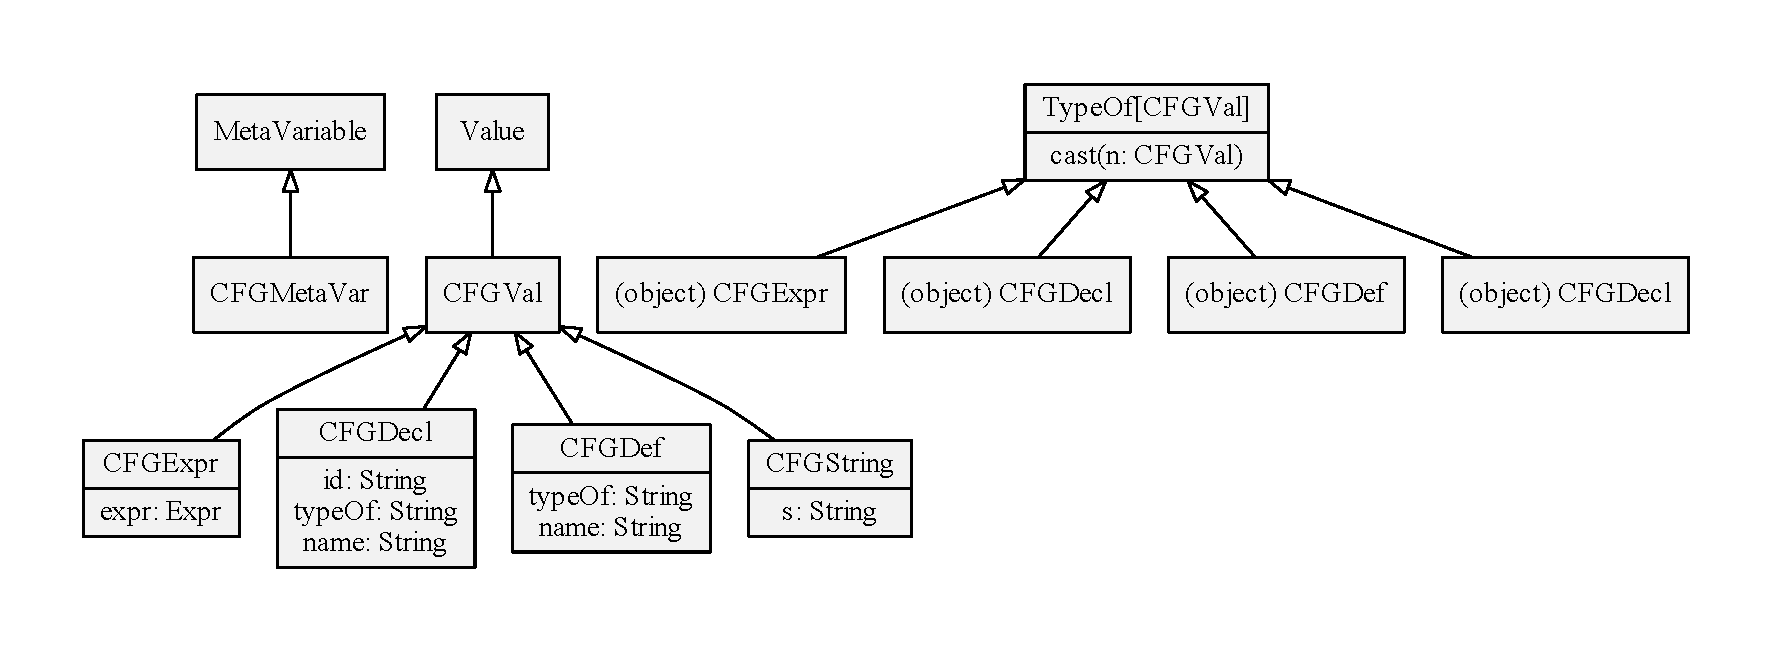
\includegraphics[scale=0.65]{data/merge_types}
~\\~\\Figure IV.1 - Concrete implementation of the generic types of the CTL part
\end{center}

\section{Labelize our nodes}

\subsection{Patterns}

\paragraph{}
\hspace{4mm}Most of the predicates we need to use were based on the idea of a pattern of code. For example, $X = 0$ is a pattern describing all the assignments to 0
of a variable to be determined (using capital-size letter means that this is a meta-variable and not a variable of the code). Using patterns, we are able 
to tell many things about a node and express many base properties. The patterns had to be able to match all kinds of entities in a code and allow for 
returning bindings between the meta-variables of the pattern and the matching values in case of success of the matching. For the same reasons as in the
previous part, we determined that we needed :

\vspace{1.5mm}
\begin{itemize}
\item patterns for expressions : ExprPattern\vspace{1mm}
\item patterns for declarations : DeclPattern\vspace{1mm}
\item patterns for string values : StringPattern\vspace{1mm}
\end{itemize}

\paragraph{}
\hspace{4mm}For expression patterns, we did not want to explore more than one level of depth of the expressions.
Deeper exploration of the expression tree would be nearly pointless for the properties we aim to assert on the CFG, moreover
some patterns may be ambiguous or more bothering to define if we explored the tree deeper (for example, $5 + x + y + 6$ can be matched in several ways by the $X + Y$ patterns, 
X and Y being meta-variables). Even if the AST generated by an expression is deterministic, which makes deep pattern matching possible, we thought it was not very clear for the user
what he would get when using deep patterns. Therefore, we introduced the AtomicExprPattern, which is only extended by leaves expressions patterns and is the only kind of ExprPattern
that can be passed as a parameter to a non-leave expression pattern. This choice is entirely reversible and has no consequence on the rest of our design.

\paragraph{}
\hspace{4mm}StringPattern and ExprPattern have in common the fact that they can be whether an UndefinedVar, which is a simple wrapper of a meta-variable that matches anything
and returns the appropriate binding, or a specific value (DefinedExpr, DefinedString). StringPattern can also be a NotString, which is comparable to a negative binding : it is a set
of forbidden values. We did not need to use such thing for ExprPatttern, but nothing in our conception prevents us from adding it later.

\paragraph{}
\hspace{4mm}Finally, DeclPattern is a bit different than the other two. It can also be an UndefinedVar, but we did not see any use-case for a DefinedDecl pattern. 
We actually only treated variable declarations, which required to have a powerful pattern-matching based on the name, the type and the assigned expression, if any.
We needed two patterns doing mostly the same thing but returning in one case a CFGDecl, and in the other case a CFGDef. Consequently, we factorized the code of those two patterns
in VarDeclMatcher. The specific behaviour of VarDefPattern and VarDeclPattern is implemented in the conversion method passed as a parameter in the constructor of VarDeclMatcher.

\begin{center}
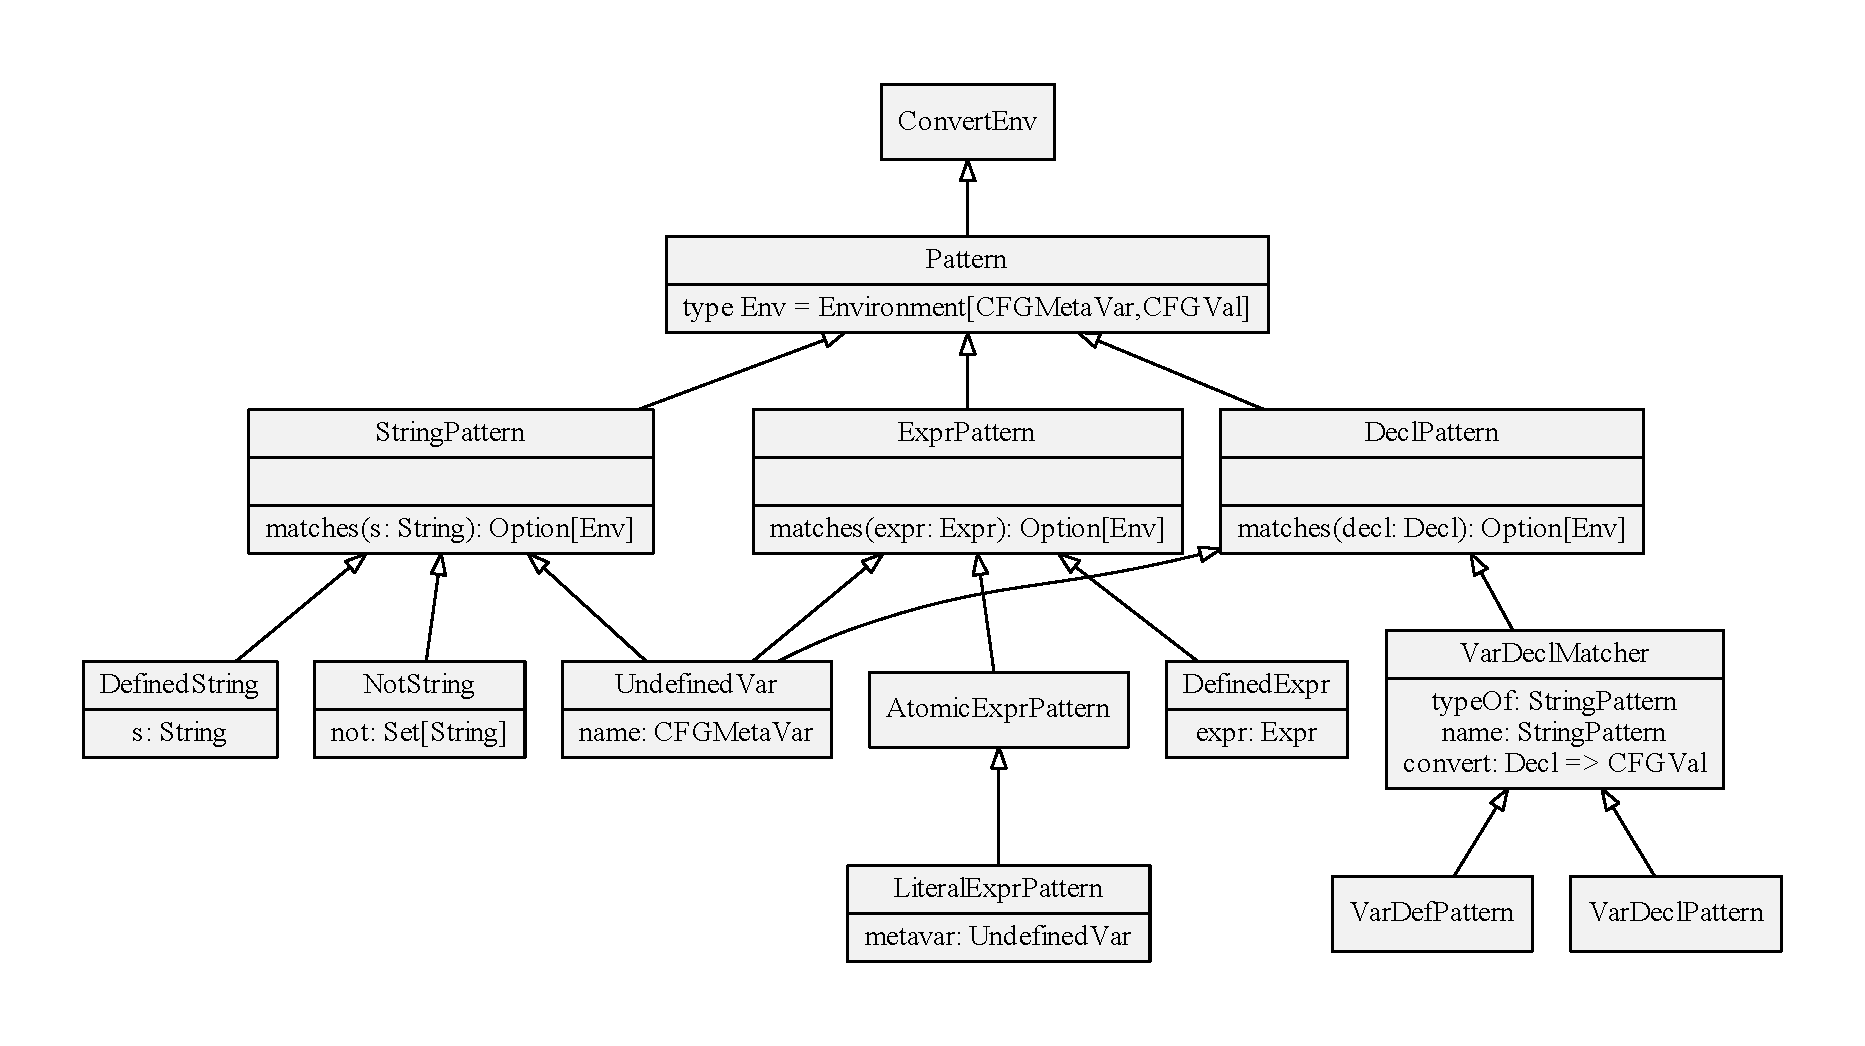
\includegraphics[scale=0.55]{data/patterns}
~\\~\\Figure IV.2 - Hierarchy of the Pattern type
\end{center}

\begin{center}
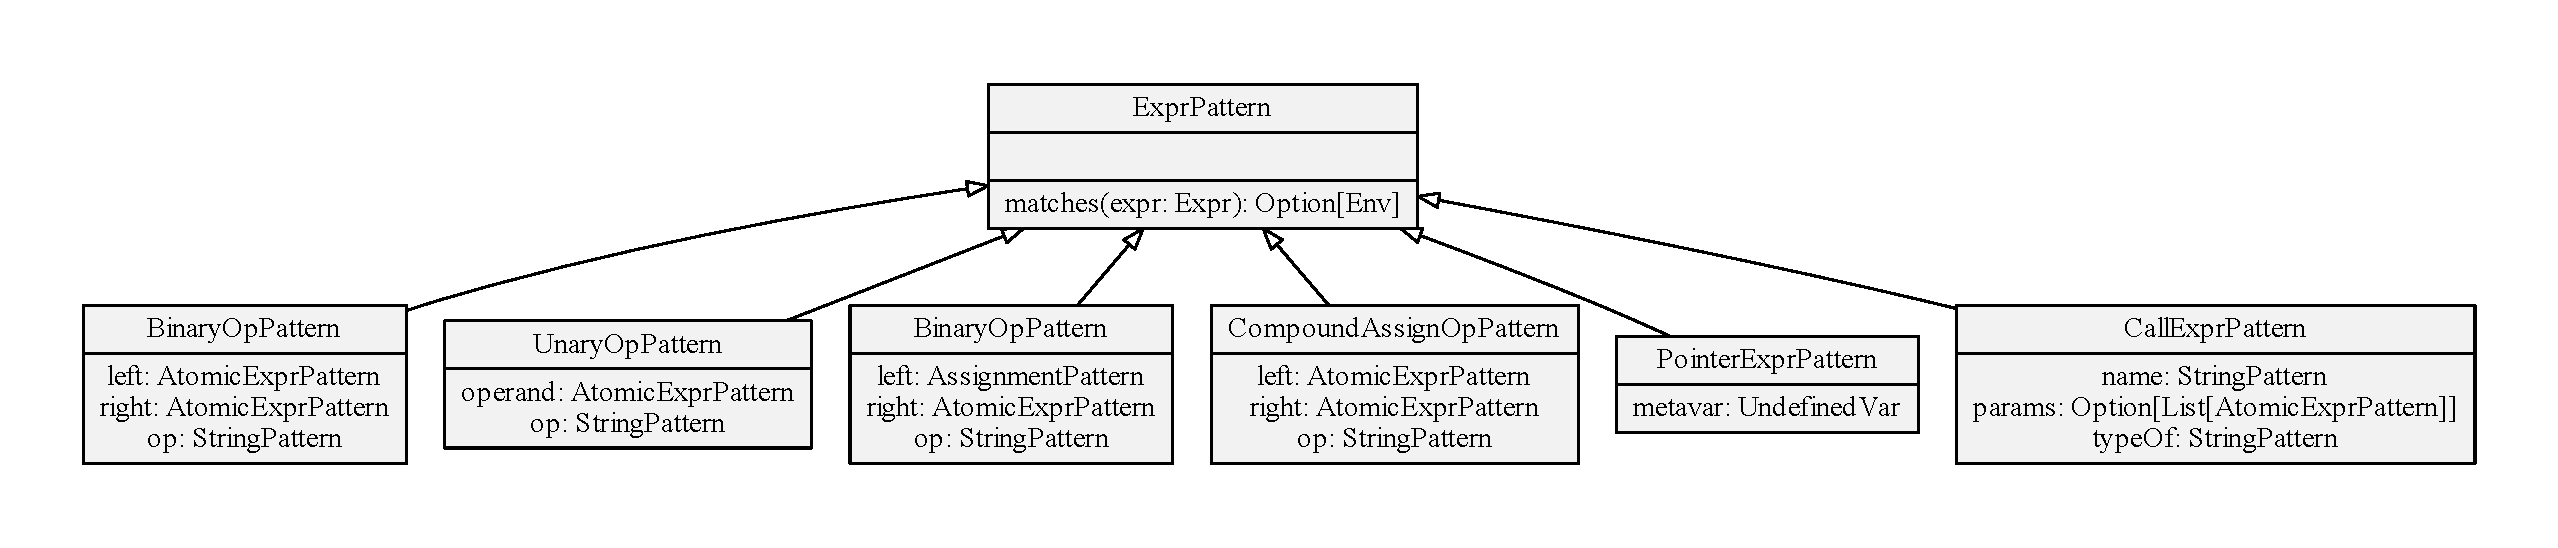
\includegraphics[scale=0.45]{data/expr_pattern}
~\\~\\Figure IV.3 - Detail of all the expression patterns
\end{center}

\subsection{Labelizers}

\paragraph{}
\hspace{4mm}Basically, our labelizers simply wrap a Pattern to add a specific semantic. Here is the list of all the labelizers, with their semantic :

\vspace{1.5mm}
\begin{itemize}
\item \textbf{IfLabelizer}, \textbf{ForLabelizer}, \textbf{WhileLabelizer}, \textbf{SwitchLabelizer}, \textbf{ExpressionLabelizer} :
all those labelizers firstly check than the node considered is of the appropriate type (respectively : If, For, While, Switch, Expression) and then if the expression
it eventually holds matches a given pattern.\vspace{1mm}
\item \textbf{VarDeclLabelizer}, \textbf{VarDefLabelizer} : match any Statement node containing a VarDecl matching a given pattern. The difference betwen those two classs is the kind of CGVal returned
in case of success (CFGDecl or CFGDef).\vspace{1mm}
\item \textbf{FindExprLabelizer} : matches any node containing at least an occurrence of a given pattern. Returns all the occurrences of the pattern in the node.\vspace{1mm}
\item \textbf{MatchesExprLabelizer} : matches any node holding an expression that exactly matches a given pattern. It returns a single value in case of success, which makes it different from FindExprLabelizer.\vspace{1mm}
\end{itemize}

\begin{center}
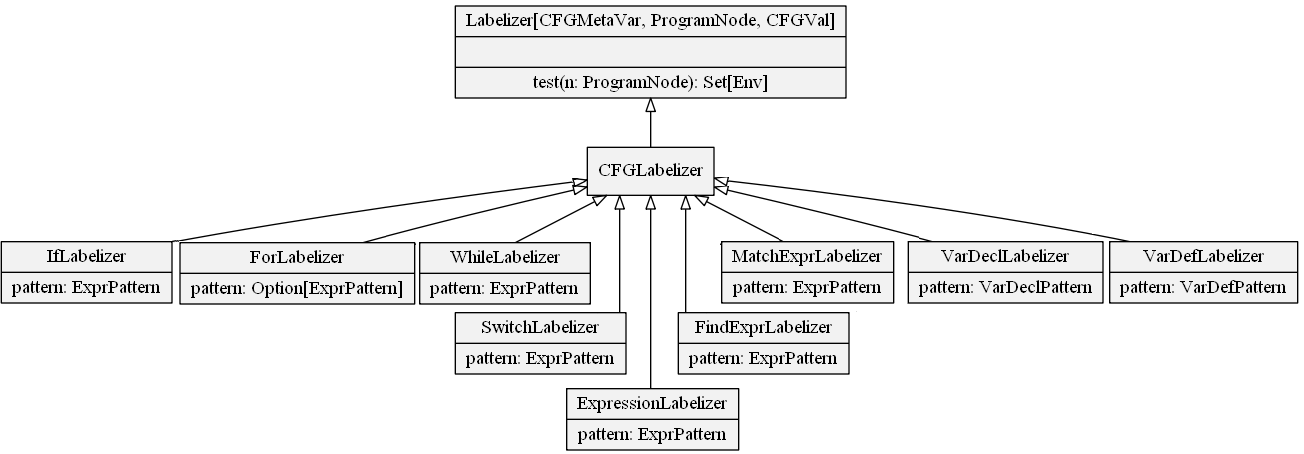
\includegraphics[scale=0.55]{data/labels.png}
~\\~\\Figure IV.4 - Detail of all the labelizers we implemented
\end{center}

\end{document}
